\input{configuration}

\title{Lecture 22 --- Transactions }

\author{Jeff Zarnett \\ \small \texttt{jzarnett@uwaterloo.ca}}
\institute{Department of Electrical and Computer Engineering \\
  University of Waterloo}
\date{\today}


\begin{document}

\begin{frame}
  \titlepage

 \end{frame}


\begin{frame}
\frametitle{Transactions}

Transactions are fundamental to database operations. 

A transaction is a grouping of operations that belong together and should be treated as an indivisible unit. 

\begin{center}
	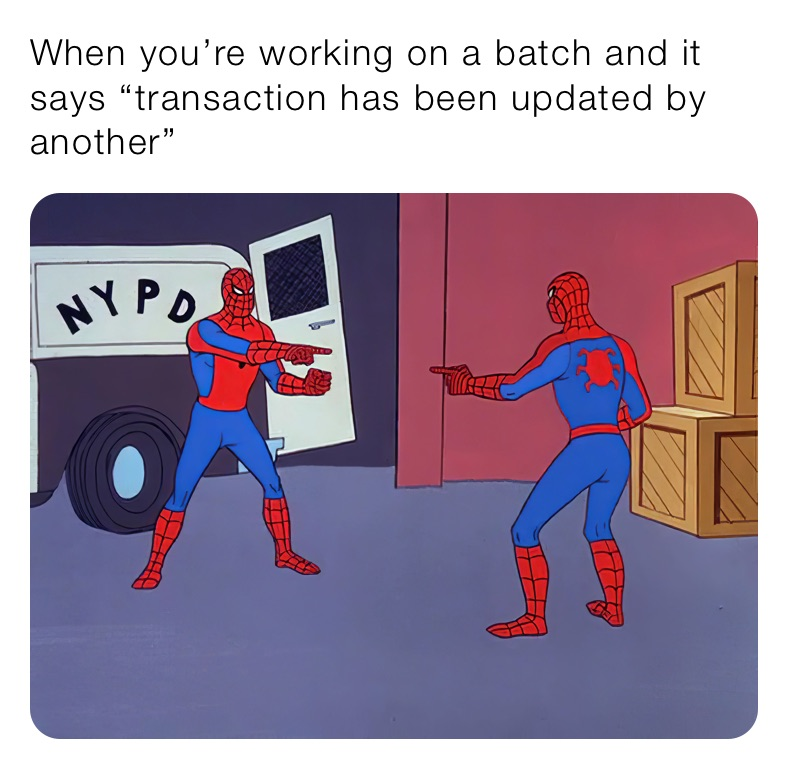
\includegraphics[width=0.4\textwidth]{images/transactions.jpg}
\end{center}

 \end{frame}


\begin{frame}
\frametitle{Transactions}


Remember \texttt{x++;}? The solution we used then was mutual exclusion.

The transaction is the database way of dealing with the need to prevent intermediate state from becoming visible.


\end{frame}

\begin{frame}
\frametitle{Transactions: VCS}

Version control systems such as git and subversion use transactions. 

This seemingly-simple use case really captures all the most important attributes of transactions, as we will see. 

Understanding transactions as a concept is easy... implementing their behaviour is harder...

You may also recall from an operating systems class that modern file systems like NTFS or HFS+ are journaled. 

\end{frame}

\begin{frame}
\frametitle{Transaction Structure}
To execute a transaction we need first to create one. 

A transaction has a begin transaction statement, then the operations to take place in the transaction, and finally an end transaction statement. 

\begin{center}
	
\includegraphics[width=0.5\textwidth]{images/rememberit.jpg}
\end{center}

\end{frame}

\begin{frame}
\frametitle{Transactions: VCS}


Execution looks something like writing down the transaction into a log, and then doing the operations in the transaction. 

When the last one is complete, mark the transaction as successful. 


\end{frame}

\begin{frame}
\frametitle{Transaction States}
\begin{itemize}
\item \textbf{Not Started}
\item \textbf{Running}
\item \textbf{Ready to Commit}
\item \textbf{Committed}
\item \textbf{Failed}
\item \textbf{Aborted}
\end{itemize}

\end{frame}

\begin{frame}
\frametitle{F is for Failure}

How might a transaction be unsuccessful? 

An error might be encountered in execution of the query.

These exceptions tend to be handled by undoing any partly-done changes.

\end{frame}

\begin{frame}
\frametitle{ACID}
Transactions should have the \alert{ACID} properties:

\begin{center}
	
\includegraphics[width=0.5\textwidth]{images/acid.jpg}
\end{center}

\end{frame}

\begin{frame}
\frametitle{ACID}
Transactions should have the \alert{ACID} properties:
\begin{itemize}
	\item \textbf{Atomicity}
	\item \textbf{Consistency preservation}
	\item \textbf{Isolation}
	\item \textbf{Durability}
\end{itemize}
\end{frame}


\begin{frame}
\frametitle{Obligatory, Mandatory, Non-Optional Bank Analogy}

It was inevitable that a bank analogy would be applied to transactions. 

The example revolves around transferring \$50 from account A to account B. 

This is a common operation: your friend buys tickets to a Metallica Concert.

\begin{center}
	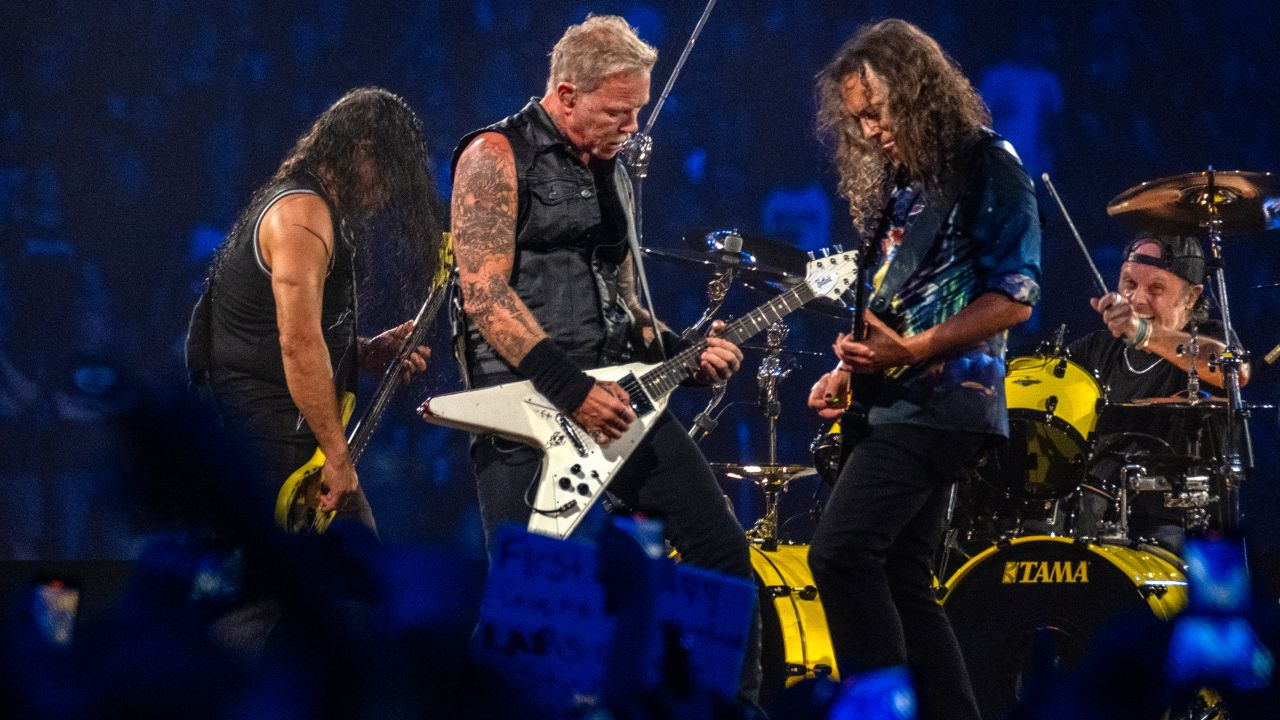
\includegraphics[width=0.7\textwidth]{images/metallica.jpg}
\end{center}


\end{frame}


\begin{frame}
\frametitle{Obligatory, Mandatory, Non-Optional Bank Analogy}
You send an electronic bank transfer to said friend in the amount of your half.  

Here's a situation where both parts need to happen for everyone to be happy. 

\end{frame}

\begin{frame}[fragile]
\frametitle{Bank Analogy Pseudocode}

\begin{verbatim}
BEGIN TRANSACTION
read A.balance
A.balance = A.balance - 50
write A.balance
read B.balance
B.balance = B.balance + 50
write B.balance
END TRANSACTION
\end{verbatim}

\end{frame}

\begin{frame}
\frametitle{Applying ACID}
If we do not have atomicity in this transaction then it is possible that some halfway completed state is revealed.

Moreover, if we have a crash at this stage, the operation is only partway complete and that is undesirable. But we already wrote A.balance?!

\end{frame}


\begin{frame}
\frametitle{Atomicity}

The way we prevent this problem is the same way that NTFS does it: log file. 

The transaction steps are written in the log file before they are executed. 

The transaction is treated like a checklist: after each operation is done we check off the box next to the operation and then we may proceed to the next. 

\begin{center}
	
\includegraphics[width=0.5\textwidth]{images/step1.png}
\end{center}

\end{frame}


\begin{frame}
\frametitle{Atomicity}

If there is a crash and we have an inconsistent state, we can use the log to go backwards and undo the partially complete operation.

We might even be able to pick up where we left off and finish it. 

Either way, we can't leave it half done: forward or back, we have to be at one consistent state or another.


\end{frame}

\begin{frame}
\frametitle{Consistency}
There aren't any sort of foreign key or unique key rules here.

But: the sum of account A and account B must remain the same after the transaction is done. 

If that is not true, then something is wrong and money has gone missing or been created out of thin air. 

\end{frame}

\begin{frame}
\frametitle{Consistency}

\begin{center}
	
\includegraphics[width=0.6\textwidth]{images/moneyprinter.jpg}
\end{center}

Destroying and creating money are the job of the central banks and they get very upset when you try to do it yourself at home. 

\end{frame}

\begin{frame}
\frametitle{Other Consistency Rules}

There could exist other consistency rules in this system that come in to play. 

For example, the balance may be required to be non-negative. 

So if you attempted to transfer \$50 to someone from an account that contains only \$31.25 then the transaction will not succeed.

The consistency check that says balance must be greater than or equal to zero will be violated.

\end{frame}

\begin{frame}
\frametitle{Isolation}

As we know, the same data is being accessed by multiple threads in a C program, there is the possibility that an error will result. 

An unlucky interleaving of statements could happen here as well. 

\begin{center}
	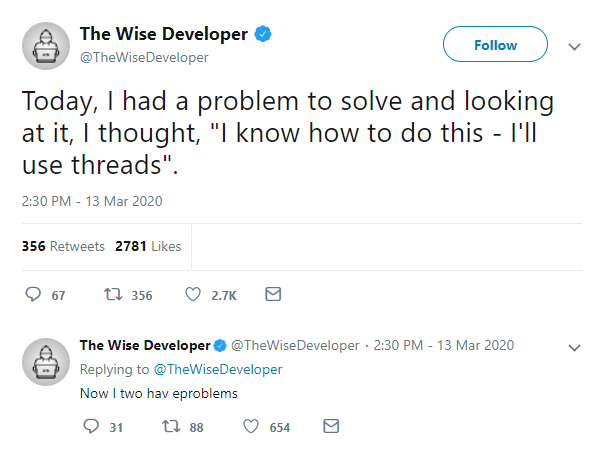
\includegraphics[width=0.5\textwidth]{images/twoproblems.png}
\end{center}

\end{frame}

\begin{frame}
\frametitle{Isolation}


Simple solution: we can just do transactions one at a time. 

Isolation is a very complex subject that will be the subject of the next lecture.

\end{frame}

\begin{frame}
\frametitle{Durability}
Finally, once the transaction has reached the end statement and it is ready to commit, that change should be permanently reflected in the data on disk. 

For a transaction to be truly durable it means that if the system crashes at this point, the transaction's changes will not be lost. 

Either: (1) the data has already been written to disk; or 

(2) the information already written to disk is sufficient that we could redo the changes if the system is restarted after a failure.


\end{frame}

\begin{frame}
\frametitle{Stable Storage}

For a transaction to be really considered permanent, it might not actually be enough just to write it out to disk. 

Disk is not volatile storage and data on disk will be preserved if the power goes out or the server process crashes or something. 

But that does not account for another mode of failure: hard drive death! 

Hard drives can and do die at the worst possible times.


\end{frame}


\begin{frame}
\frametitle{Stable Storage}

A further level of storage beyond non-volatile is called \alert{stable storage} which they define as where data can never get lost. 

\begin{center}
	
\includegraphics[width=0.5\textwidth]{images/forever.jpg}
\end{center}

Never is somewhat exaggerated: no matter how many forms of storage you have, a nuclear war will probably get them all (or at least all of us). 

\end{frame}


\begin{frame}
\frametitle{Stable Storage}

The point of stable storage, though, is to be sure that even the failure of nonvolatile storage is not sufficient for data to get lost.

A transaction isn't really truly durable until it has been written into the stable storage.


\end{frame}

\begin{frame}
\frametitle{Stable Storage}
In real life where we don't have infinite money and plan for more reasonable scenarios than nuclear armageddon or the rise of Skynet...

Strategy 1 is the RAID array (redundant array of independent disks) so the failure of any individual disk does not result in data loss. 

The next strategy is backups! Buying a backup drive today is like a tenth of the price of sending your dead drive out for recovery. 

\end{frame}

\begin{frame}
\frametitle{Back it Up}

For best results, the data you consider important should be backed up and there should also be off-site backups. 


For the strictest possible definition, a transaction is really only durable when it is not only written to stable storage and the backups are updated too.

\end{frame}


\begin{frame}
\frametitle{Atomicity and Durability}

The log file is the most important key to the usual approach. 

The more detail is written into the log file, the more options we have for dealing with a failure of the transaction if it occurs. 

The trade-off here is of course the size of the log and the amount of time spent maintaining that log. 


\begin{center}
\begin{tabular}{|l|l|l|l|l|l|}\hline
	\textbf{Transaction ID} & \textbf{Relation} & \textbf{ID} & \textbf{Attribute} & \textbf{Old Value} & \textbf{New Value}\\ \hline
	385 & account & 8675309 & balance & 5000.00 & 4950.00 \\ \hline
\end{tabular}
\end{center}



\end{frame}

\begin{frame}
\frametitle{Alternative Atomicity}

Another way that we can get atomicity is the ZFS (A file system developed by Sun Microsystems) approach. 

In this case when a transaction is to be executed, a copy of the data is made. 

The copy is modified, and if the transaction runs to completion, then the copy replaces the original data. 


\end{frame}

\begin{frame}
\frametitle{Atomicity and Durability}

Getting to the state ``committed'' actually means that the transaction is not only completed. 

It also means it is written out to disk in such a way that if the system crashes now that transaction will not get lost. 

That is an important rule to hold to because without it we could check off an item as done when it is not actually done.

\end{frame}

\begin{frame}
\frametitle{Managing the Log}

If the transaction succeeds and is committed, it can be removed from the log. 

\begin{center}
	
\includegraphics[width=0.5\textwidth]{images/finalexam.jpg}
\end{center}


\end{frame}

\begin{frame}
\frametitle{Managing the Log}

This keeps the log file size reasonable. 

In many cases the log contains only the in-progress transactions. 

A quick glance at the log file will tell the database server on boot up whether any transactions were in progress at the time of crash.


\end{frame}

\begin{frame}
\frametitle{Commit is Final}

Once a transaction is committed, we cannot cancel or roll back its effects. 

In the words of Lady MacBeth: ``What's done is done and cannot be undone.'' 

You can return the system to an equivalent state to the before by executing a \alert{compensating transaction}.

 Compensating transactions are not always possible when information is tossed away such as a deletion...

\end{frame}

\begin{frame}
\frametitle{Something went wrong...}

Suppose that a transaction does not succeed. 

There are now two ways forward from the aborted state. 

The first is to re-try the transaction. 

\begin{center}
	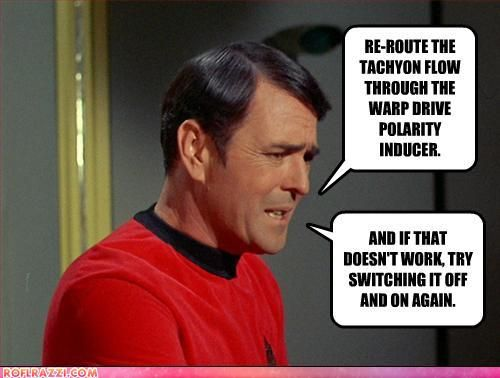
\includegraphics[width=0.4\textwidth]{images/tryagain.jpg}
\end{center}


\end{frame}

\begin{frame}
\frametitle{Something went wrong...}


Sometimes the transaction failed due to temporary circumstances, network disruption being one such example. 

As we will see, transactions sometimes interfere with each other a bit and that can cause one of them to need to start over again. 

The transaction, having been aborted, is assigned a new number.

\end{frame}

\begin{frame}
\frametitle{Failure = Death}

The alternative is to kill the transaction, which is really the same as giving up. 

Giving up is mandatory if the operation in question failed due to some unrecoverable error such as trying to violate a constraint.

\begin{center}
	
\includegraphics[width=0.3\textwidth]{images/physics.png}
\end{center}

\end{frame}

\begin{frame}
\frametitle{Failure = Death}

 An error of some sort will be returned the requesting program/client to indicate the failure. 
 
 Once that happens it is out of the database server's hands and purview.
\end{frame}



\begin{frame}
\frametitle{Console and Network}

There's a problem with external writes: i.e. making results available to users and other devices or individuals outside the database system. 

Once data has gone out over the network or has been printed to the console there is no way to get it back. 

The fully correct rule to handle this would be to allow no such output until the transaction is committed. 

We could write data to a temporary location until such time that is true. 


\end{frame}

\begin{frame}
\frametitle{Intermediate State}

Sometimes the state of an external write of some sort is fairly indeterminate: what happens if we aren't sure whether the data was sent to the printer?

Sometimes, we actually want to show the status of a transaction to a user. 


Users love progress bars...

\end{frame}







\end{document}

